%%%%%%%%%%%%%%%%%%%%%%%%%%%%%%%%%%%%%%%%%%%%%%%%%%%%%%%%%%%%%%%%%
%%%  The truth is out there and also in Twitter: analyzing Events via Name Entity Extraction %%%
%%%%%%%%%%%%%%%%%%%%%%%%%%%%%%%%%%%%%%%%%%%%%%%%%%%%%%%%%%%%%%%%%

\documentclass{sig-alternate}



\newcommand{\superscript}[1]{\ensuremath{^{\textrm{#1}}}}

\usepackage[hyphens]{url}
\usepackage{textcomp}
\usepackage{color}
\usepackage{listings}
\usepackage{multirow}
\usepackage{mathtools}
\usepackage{graphicx}
\usepackage{fancyvrb}
\usepackage{amsmath}
\usepackage{graphicx}
\usepackage[font=small,labelfont=bf]{caption}
\setcounter{MaxMatrixCols}{20}
\usepackage{pbox}

% listing styles
\lstset{numbers=left, numberstyle=\tiny,basicstyle=\ttfamily\scriptsize, tabsize=2, keywordstyle=\underbar, stringstyle=\small, backgroundcolor=\color[gray]{0.94}, framexleftmargin=2pt}
\lstdefinestyle{rdfa}{numberblanklines=true, morekeywords={}}

% Turtle box
\definecolor{olivegreen}{rgb}{0.2,0.8,0.5}
\definecolor{grey}{rgb}{0.5,0.5,0.5}
\lstdefinelanguage{ttl}{
sensitive=true,
morecomment=[l][\color{grey}]{@},
morecomment=[l][\color{olivegreen}]{\#},
morestring=[b][\color{blue}]\",
keywordstyle=\color{cyan},
morekeywords={version,owl,rdf,rdfs,xml,xsd,dbpedia,dbo,str,sso,scms,fr,ld}
}
\lstset{
        basicstyle=\ttfamily\scriptsize,
        upquote=true,
        showspaces=false,
        showstringspaces=false,
        showtabs=false,
        tabsize=2,
        frame=none,
        breaklines,
        numbers=none,
        framexleftmargin=2mm,
        xleftmargin=2mm,
}

\newcommand{\hilight}[1]{\colorbox{yellow}{#1}}
\newcommand{\todo}[1]{\colorbox{red}{#1}}

%\permission{Copyright is held by the International World Wide Web Conference Committee (IW3C2). IW3C2 reserves the right to provide a hyperlink to the author's site if the Material is used in electronic media.}
%\conferenceinfo{WWW'14 Companion,}{April 7--11, 2014, Seoul, Korea.}
%\copyrightetc{ACM \the\acmcopyr}
%\crdata{978-1-4503-2745-9/14/04.\\
%http://dx.doi.org/10.1145/2567948.2579326}
%\\Include the http://DOI string/url which is specific for your submission and included in the ACM rightsreview confirmation email upon completing your IW3C2 form}

%\clubpenalty=10000
%\widowpenalty = 10000

%%%%%%%%%%%%%%%%%%%%%%%%%%%%%%%
%%%  Beginning of document  %%%
%%%%%%%%%%%%%%%%%%%%%%%%%%%%%%%

\begin{document}

%\title{Named Entities for Analyzing Events in Twitter Stream}
\title{The Truth is out there and also on Twitter: \\ Analyzing Events via Name Entity Extraction}

\numberofauthors{4}
\author{
\alignauthor Jos\'e Luis Redondo Garc\'ia\\
	\affaddr{EURECOM}\\
	\affaddr{Sophia Antipolis, France}\\
	\email{redondo@eurecom.fr}
\alignauthor Giuseppe Rizzo\\
	\affaddr{Universit\`a di Torino, Turin, Italy}\\
	\affaddr{EURECOM, Sophia Antipolis, France}\\
	\email{giuseppe.rizzo@di.unito.it}
\and
\alignauthor Laurens De Vocht\\
    \affaddr{Ghent University - iMinds}\\
    \affaddr{Ghent, Belgium}\\
    \email{laurens.devocht@ugent.be}
\alignauthor Rapha\"el Troncy\\
	\affaddr{EURECOM}\\
	\affaddr{Sophia Antipolis, France}\\
	\email{raphael.troncy@eurecom.fr}	\\
}

\maketitle

%%%%%%%%%%%%%%%%%%
%%%  Abstract  %%%
%%%%%%%%%%%%%%%%%%

\begin{abstract}

Social platforms open a window to what is happening in the world in real-time: people are constantly sharing and reporting their experiences and feelings concerning any kind of event. Such information can be programmatically collected and analyzed in order to get extra insights about what is happening out there. However, the volume, velocity and variety of the information make tough the task of extracting stories from social media streams. In this paper, we present a general framework to automatically mine social platforms, providing to journalists a set of headlines and complementary information that summarize the most important topics inside a given time interval. The approach consists of collecting tweets, grouping them in time-slots and further analyzing them through deduplication, name entity extraction, clustering, and popularity ranking techniques. The final output is a temporally ordered list of topics that aim to summarize the most relevant insights about a target event. 

\end{abstract}

% A category with the (minimum) three required fields
\category{H.3}{Information Storage and Retrieval}{Content Analysis and Indexing}

\keywords{Topic Generation, Name Entity Extraction, Event Detection}

%%%%%%%%%%%%%%%%%%%%%%
%%%  Introduction  %%%
%%%%%%%%%%%%%%%%%%%%%%

\section{Introduction}
\label{sec:introduction}
The amount of data shared on the Web is exponentially increasing. With the wide adoption of social platforms, millions of users are constantly interacting and generating comments about what is happening around the world in great detail: giving opinions, providing videos and photos, linking to resources where extra information can be found, etc. A set of innovative analysis techniques intend to use those spread pieces of information for providing professionals with insightful highlights and the users a novel experience about appealing stories happening right now.

The understanding of a particular user generated post could benefit from the application of semantic analysis methods, but this is still a very challenging task specially considering the informal nature of most of the social platforms. One of the available approaches consist in using Named Entity Recognition (NER) over the textual information attached to particular video fragment. Those techniques are an essential component within the Information Extraction field that focus on: identifying atomic information units in texts, named entities; classifying entities into predefined categories (also called context types) and linking to real world objects using web identifiers (Named Entity Disambiguation). A growing number of APIs provide such a service, like AlchemyAPI\footnote{\fontsize{8pt}{1em}\selectfont \url{http://www.alchemyapi.com/}} or DBpedia Spotlight\footnote{\fontsize{8pt}{1em}\selectfont \url{http://spotlight.dbpedia.org/}}. Some studies have conducted experiments in how to apply those techniques over the noisy and informal 140 character messages coming from Twitter, like in Ritter et al.~\cite{Ritter2011} where they have probed to get very promising results by leveraging in tweets redundancy and exploiting Freebase dictionaries as a source of distant supervision. 

The massive amount and steady increase of heterogeneous data shared on social platforms has attracted the interest of different research communities. Status updates or tweets enable people to share their activities, feelings, emotions and conversations, opening a window to the world in real-time. Making sense out this amount of data is an extremely challenging task due to its heterogeneity (media items mixed with textual data) and dynamics making often short-lived phenomena. A growing number of commercial tools and academic research approaches try to partially collect and analyze this data in order to make sense of it. Capturing life moments and building narratives using social platforms is, for example, the goal of Storify\footnote{\url{http://storify.com}} where the creators aim to investigate the interaction between event stories and the role of social networks that tell them: \textit{(i)}~sorting and organizing the items of an experience similar to the elements of a story, \textit{(ii)}~communicating and discussing strategies on how to guide a user towards an intended experience. The overall storytelling creation is supervised by the user who composes a story based on streams of news coming through social platforms such as Twitter and YouTube. Generating the big picture from these streams is also the objective of Storyful\footnote{\url{http://storyful.com}}. This application enables the user to navigate through the story created by other users or to create his own, aggregating content from different social platforms. While these two approaches position the role of a social platform as a container of fresh and breaking news items, they are leveraging on the user interaction that defines the summary creation as a supervised task. A disruptive innovation has been recently revealed by Mahaya\footnote{\url{http://mahaya.co}} which proposes an automatic crowd storyfication of the 12/12/12 concert\footnote{\url{http://121212.mahaya.co}}. In this example, the highlights of the concert corresponding to social media spikes when performers appeared are emphasized with images collected from Instagram, and microposts collected from Twitter. Other approach trying to recreate stories from a multimedia oriented perspective is ~\cite{Rizzo2012}, where a generic media collector for retrieving multimedia items is proposed for illustrating daily life moments shared on social platforms. A common schema aligns the search results of numerous social platforms making possible to access to a wider set of social status. In~\cite{Milicic2013} this approach is extended by adding to the codebase the temporal analysis and the cluster operations, and finally in~\cite{Milicic2013b} the authors put into practice the idea of automatic summarization through visual galleries focusing more on the adequate displaying of clusters for topic visualization. 

For the particular case of Twitter, ~\cite{Aiello} compares six topic detection method on three different datasets related to mayor events for probing that, apart of the nature of the event, the volume of activity over time, the sampling procedure and the pre-processing of the data, also the detection techniques greatly affect the quality of detected topics. Finally, in ~\cite{Schifferes} the authors elaborate on the relevance and utility of those analysis from a journalist point of view.

%%%%%%%%%%%%%%%%%%
%%%  Approach  %%%
%%%%%%%%%%%%%%%%%%

\section{Approach}

We describe the steps applied over the a stream of status coming from Twitter in order to select and highlight main topics about high coverage events. To reconstruct the topics that better illustrate a particular fact being discussed, we apply different techniques that go from collection and normalization of the tweets related with the event to name entity extraction an clustering, in order to infer which are the most relevant aspects that the crow has been commenting about.

The complete processing workflow takes as input a set of keywords which evoke the event to track, a list of Twitter user accounts, and the start and end times for the collection task. Of course we assume that the studied event has a minimal presence and coverage on the Web to ensure that there is a sufficient and illustrative Twitter activity that allows to reconstruct what is happening in there. 

The output of the algorithm is a temporally ordered list of relevant topics for the given event, which in turn contain a set of more detailed attributes that are further explained in Section~\ref{sec:expansion}. Our hypothesis states that this set of event topics provides a set of valid headlines and complementary information that summarize the most important facts behind that particular story. 

\subsection{Tweet Collection}

The tweets used as input for this approach are extracted by using the Twitter streaming API \footnote{\fontsize{8pt}{1em}\selectfont \url{https://dev.twitter.com/docs/streaming-apis}} from a set of predefined list of keywords and user accounts. For making easier this task we have used an already existing tool available in here\footnote{\fontsize{8pt}{1em}\selectfont \url{https://github.com/socialsensor/twitter-dataset-collector}}. The tweets obtained are represented following a JSON schema that has been simplified for reduce the complexity the subsequent steps of the analysis. Also, a near-deduplication process is launched in order to group tweets with the same textual content so we can consider them together in the following steps.

\subsection{Temporal groping and Named Entity Extraction}

Before passing to the next step, we have sliced the entire tracking time period into smaller slots where the different tweets are aligned to. This time dimension is one of the key aspect of an event, but it is strongly dependent on the nature of the event and the consumption needs of the person that aims to track the event. Due to such difficulties in successfully deciding on the time-slot's duration decision, we have decided to assume this number as a external parameter that has to be chosen in advance for fitting as well as possible to the particular scenario. Finally we have discarded the status published outside the boundaries of the total interval and generated time ordered groups of tweets that will be analyzed in order to discoverimportant facts about the studied event.

For each status retrieved, we perform named-entity recognition over the corresponding tweet using the NERD framework~\cite{Rizzo2012}. In our experiment the language of the tweets is restricted to English but NERD supports other languages. The output of this phase is a list of tweets with its corresponding entities annotated using the NERD ontology\footnote{\fontsize{8pt}{1em}\selectfont \url{http://nerd.eurecom.fr/ontology/nerd-v0.5.n3}}, and include relevance scores obtained from the involved extractors. 

\subsection{Named Entity Clustering }
\label{sec:expansion}

Once the Named Entities have been obtained, a first clustering operation is performed over the tweets belonging to each time-slot, in order to determine which are the most frequent entities in them. First, we iterate over all the available disambiguation URLs for finding how many different entities are available, and then for each detected URL we attached the list of tweets that have mentioned it at least once. Note that the same tweet can appear under different entity clusters. At a first glance, those entities constitute a primitive way of generating topics about the studied event, and the cardinality of the number of tweets associated to them gives an idea about their importance. Figure~\ref{fig:EntityCluster} shows in more detail this operation: a set of different topics corresponding to named entities have been extracted and ordered according tho the number of tweets in which they appear.

\begin{figure}[h!]
\centering
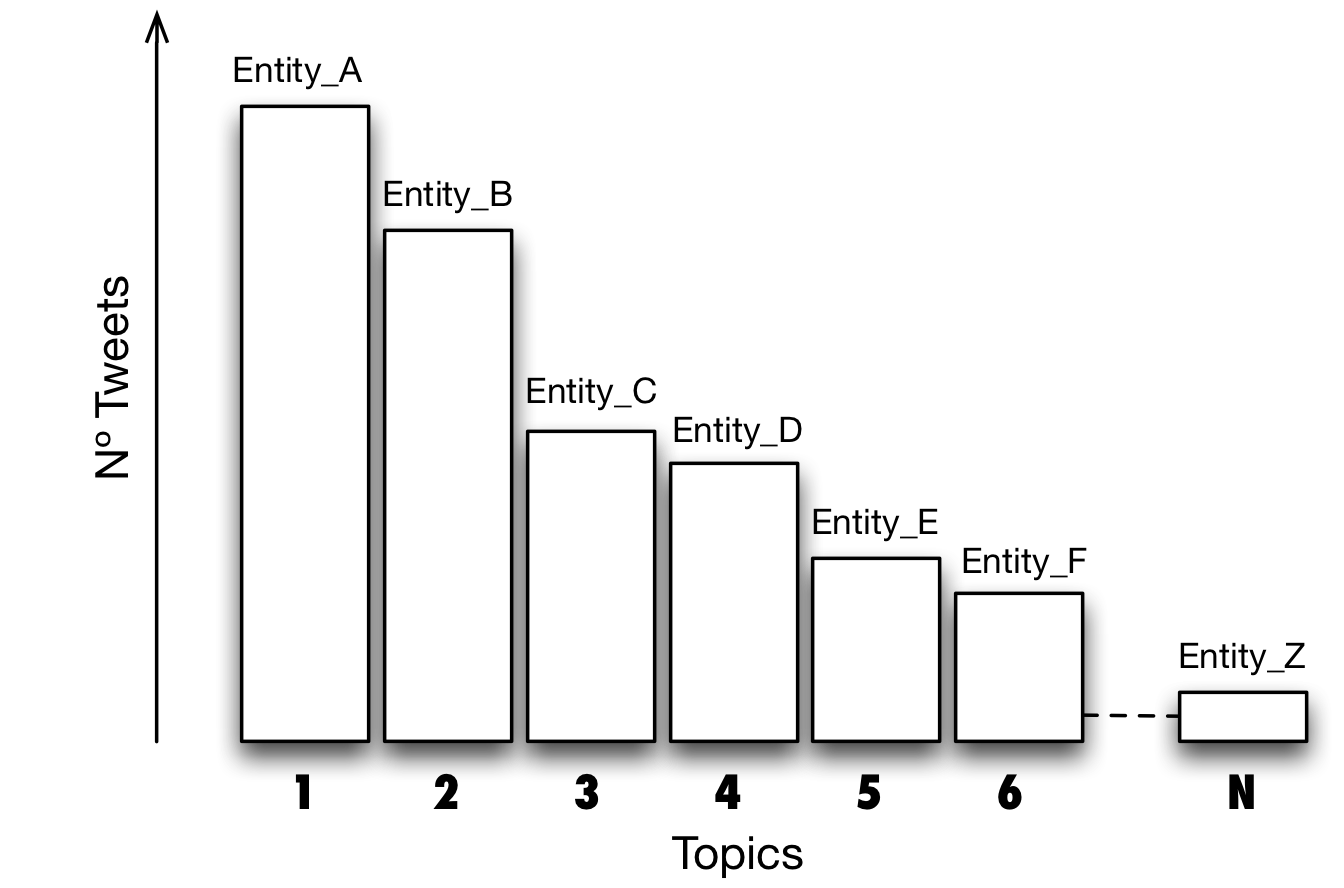
\includegraphics[width=0.4\textwidth]{figure/EntityCluster.png}
\caption{Clustering Named Entities according to their frequency in the Tweets corpora.}
\label{fig:EntityCluster}
\end{figure}

\subsubsection{Hierarchical clustering}

Next step consists of executing a cluster analysis method that builds a hierarchy of groups were certain elements are progressively merged together because they present similar characteristics. This particular implementation follows an agglomerative "bottom up" approach: each pair of clusters with similar characteristics are merged together. In order to decide which ones should be combined, we have defined a measure of similarity between different clusters based on the notion of sharing a significant amount of tweets. We iterate over all the possible pairs of clusters available in the time slot, including the new ones that are being created during the process. The process stops when no more candidate pairs are found to be merged. 

\begin{equation}
\begin{split}
\forall A, B \in Topic_{Entity}, Sim (A,B) =\frac{\left | tweets(A) \cup  tweets(b) \right |}{\left | tweets(A) \cap  tweets(b) \right |} \\
Delete(A, B) \wedge Create(C) \Leftrightarrow  Sim (A,B) > Threshold \\
C= \text{tweets(A)} \cup \text{tweets(B)}
\end{split}
\end{equation}


In Figure~\ref{fig:Hierarchical_Cluster} we observe how the clusters corresponding to \textit{Entity\_C} and \textit{Entity\_D} are combined together since the last contains a high percentage of the tweets from the first. The result is a new cluster labelled with both original entities that contains the union of the tweets coming from both them.

\begin{figure}[h!]
\centering
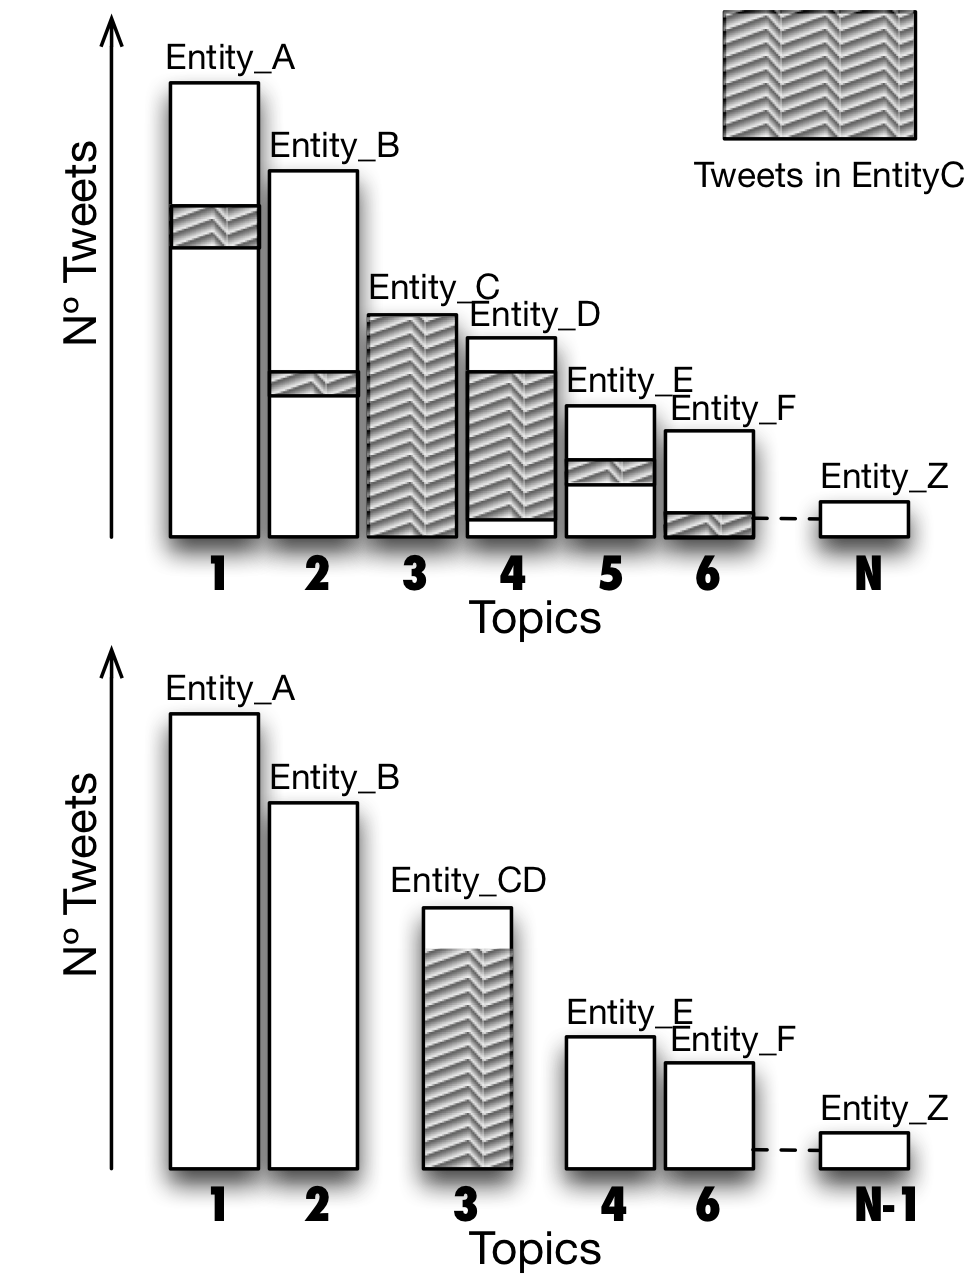
\includegraphics[width=0.4\textwidth]{figure/Hierarchical_Cluster.png}
\caption{Applying hierarchical clustering over entity clusters according to tweets coexistence.}
\label{fig:Hierarchical_Cluster}
\end{figure}

\subsubsection{Inverse Frequency Ranking}

The topics obtained so far have been ordered by taking into account the number of tweets where the corresponding entities have been found. However, the fact that an entity has an higher frequency in the entire corpora does not mean it is more relevant for that certain period of time. In many cases, the most repeated words are indeed the more general ones and therefore are not suitable for characterizing the small stories inside the whole event. In order to take in consideration this phenomena, we introduce an inverse topic frequency measure that intends to reflect how discriminating is a certain cluster inside the context of the entire set of tweets. 
Consequently, the relevance score increases proportionally to the number of tweets that contains a certain entity, but is offset by the frequency of the topic's tweet in the rest of clusters, which helps to control for the fact that some entities are more common than others. The implemented logic is summarized in the following equation:

\begin{equation}
\text{idf}(e, Slot) =\frac{N_{topics}}{\left | x\in Topics: \left | \text{tweets}(e)\cap \text{tweets}(x) < T_{20}\right |\right |}
\end{equation}

For every topic notated as $e$, this formula generates a score that increases with the total number of topics inside the time-slot and decreases with the number of other topics that contains a significant amount of tweets belonging to $e$. As displayed in Figure~\ref{fig:TF-IDF} the tweets in the cluster \textit{Entity\_D} are less spread all over the rest of topics inside that time-slot that the ones from \textit{Entity\_C}, which can be significantly found in \textit{Entity\_A},  \textit{Entity\_B} or  \textit{Entity\_E}. As consequence, \textit{Entity\_D} can be promoted against \textit{Entity\_C} for reflecting its higher discriminating rate.

\begin{figure}[h!]
\centering
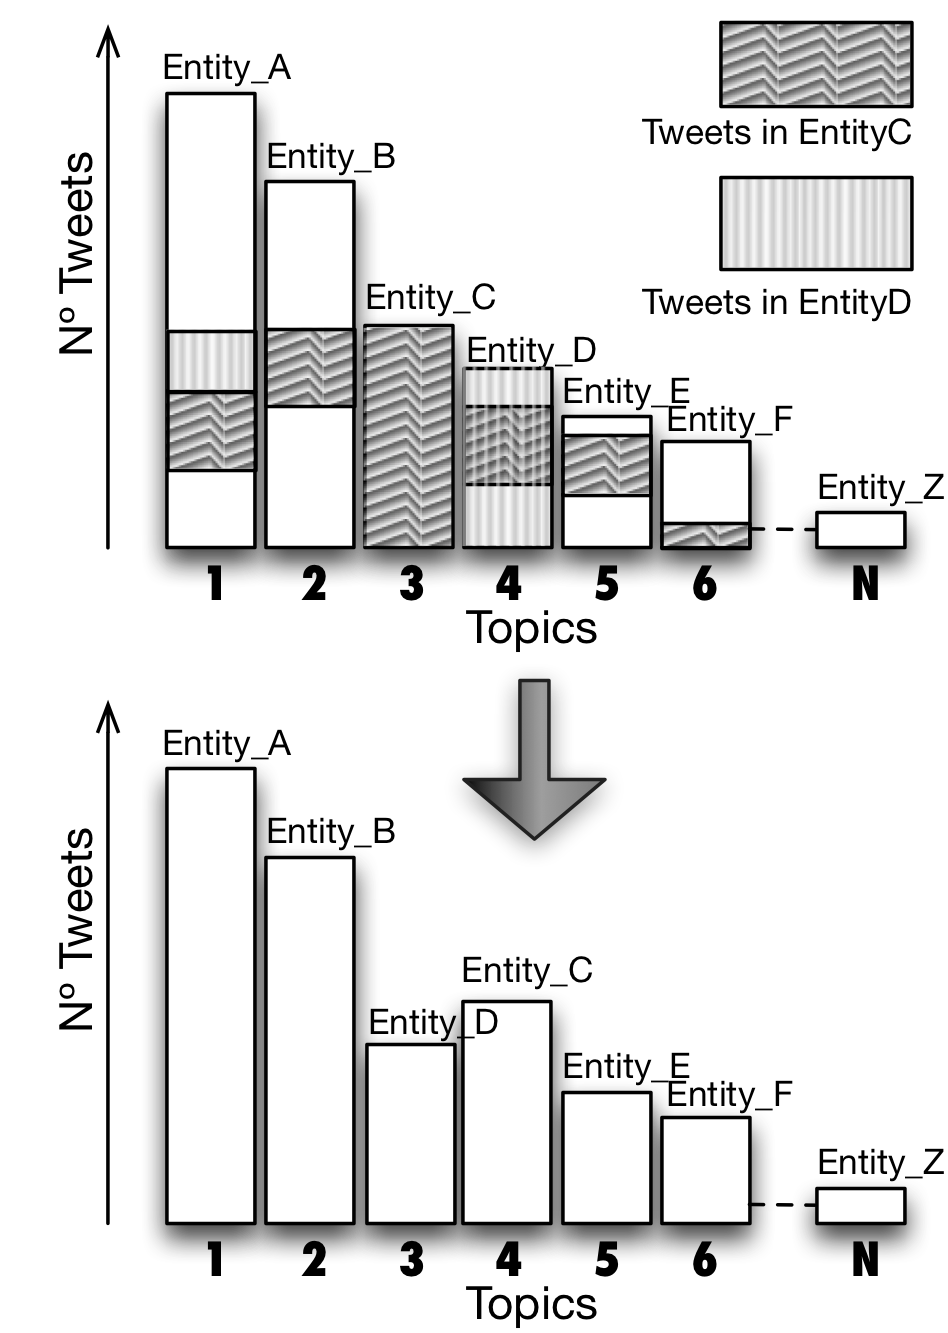
\includegraphics[width=0.4\textwidth]{figure/TF-IDF.png}
\caption{Ranking entity clusters according to inverse frequency in the rest of topics.}
\label{fig:TF-IDF}
\end{figure}

\subsubsection{Tracking Topics}

The importance of the temporal dimension in social media monitor tasks is crucial: we can not properly understand what is happening in the present without taking a look at the past. This aspect becomes even more relevant when trying to make sense out the noisy data from social networks, where the more clues we have about the present items the better results we get. It is surprising the same exact data collected for a particular time-slot can be differently interpreted depending on previous analysis about the same facts. In order to deal with this phenomena our approach implements a logic that takes into account the previous states of the detected topics when ranking and filtering them. 

In particular, we take into account two different features: the variation in the topic's tweet frequency from the former state to the current one, and a vector of scores that keeps a record about the tendency of the topic during the last states and is updated after every iteration.

\begin{equation}
\begin{split}
V_{tendency} = \left \{ s_{1} , s_{2} , s_{3} ... s_{n} \right \} :s_{n} \in (0,\mathbb{R}), \\
\left | V_{tendency}  \right |=\left | \bigcup_{n}^{0} Topic_{Entity_N}  \right |
\end{split}
\end{equation}

The final score combines together both measures as follows in order to provide the notion of topic tracking:

\begin{equation}
Trac_{n}^{t} = \left | Topic_{N} \right | *\left ( 1+\frac{\left | Topic_{N}\right |  - \left | Topic_{N-1}\right | }{max \left ( \left | Topic_{N}\right | , \left | Topic_{N-1}\right |  \right ) } \right ) * s_{n}^{t}
\end{equation}

The $V_{tendency}$ vector is updated as follows from one iteration to the other:

\begin{equation}
s_{n}^{t} = s_{n}^{t-1} *\left ( 1+\frac{\left | Topic_{N}\right |  - \left | Topic_{N-1}\right | }{max \left ( \left | Topic_{N}\right | , \left | Topic_{N-1}\right |  \right ) } \right ) * \beta
\end{equation}
\begin{itemize}
  \item A new topic T as always an tendency score $s_{t}$ equal to 1(neutral value).
  \item By default, a tendency score $s_{t}$ is reduced in a certain rate $\beta$ from one state to the following (in our approach, $\beta=0.85$).
  \item The tendency score $s_{t}$ decreases faster if the tendency is negative.
  \item The tendency score $s_{t}$ increases if the tendency in the last states has been positive enough.
\end{itemize}

In Figure~\ref{fig:Tracking} it is possible to see how the scores from time $t-1$ are combined together with the one calculated in $t$ for outputting a more accurate ranking about the importance of the topics detected.

\begin{figure}[h!]
\centering
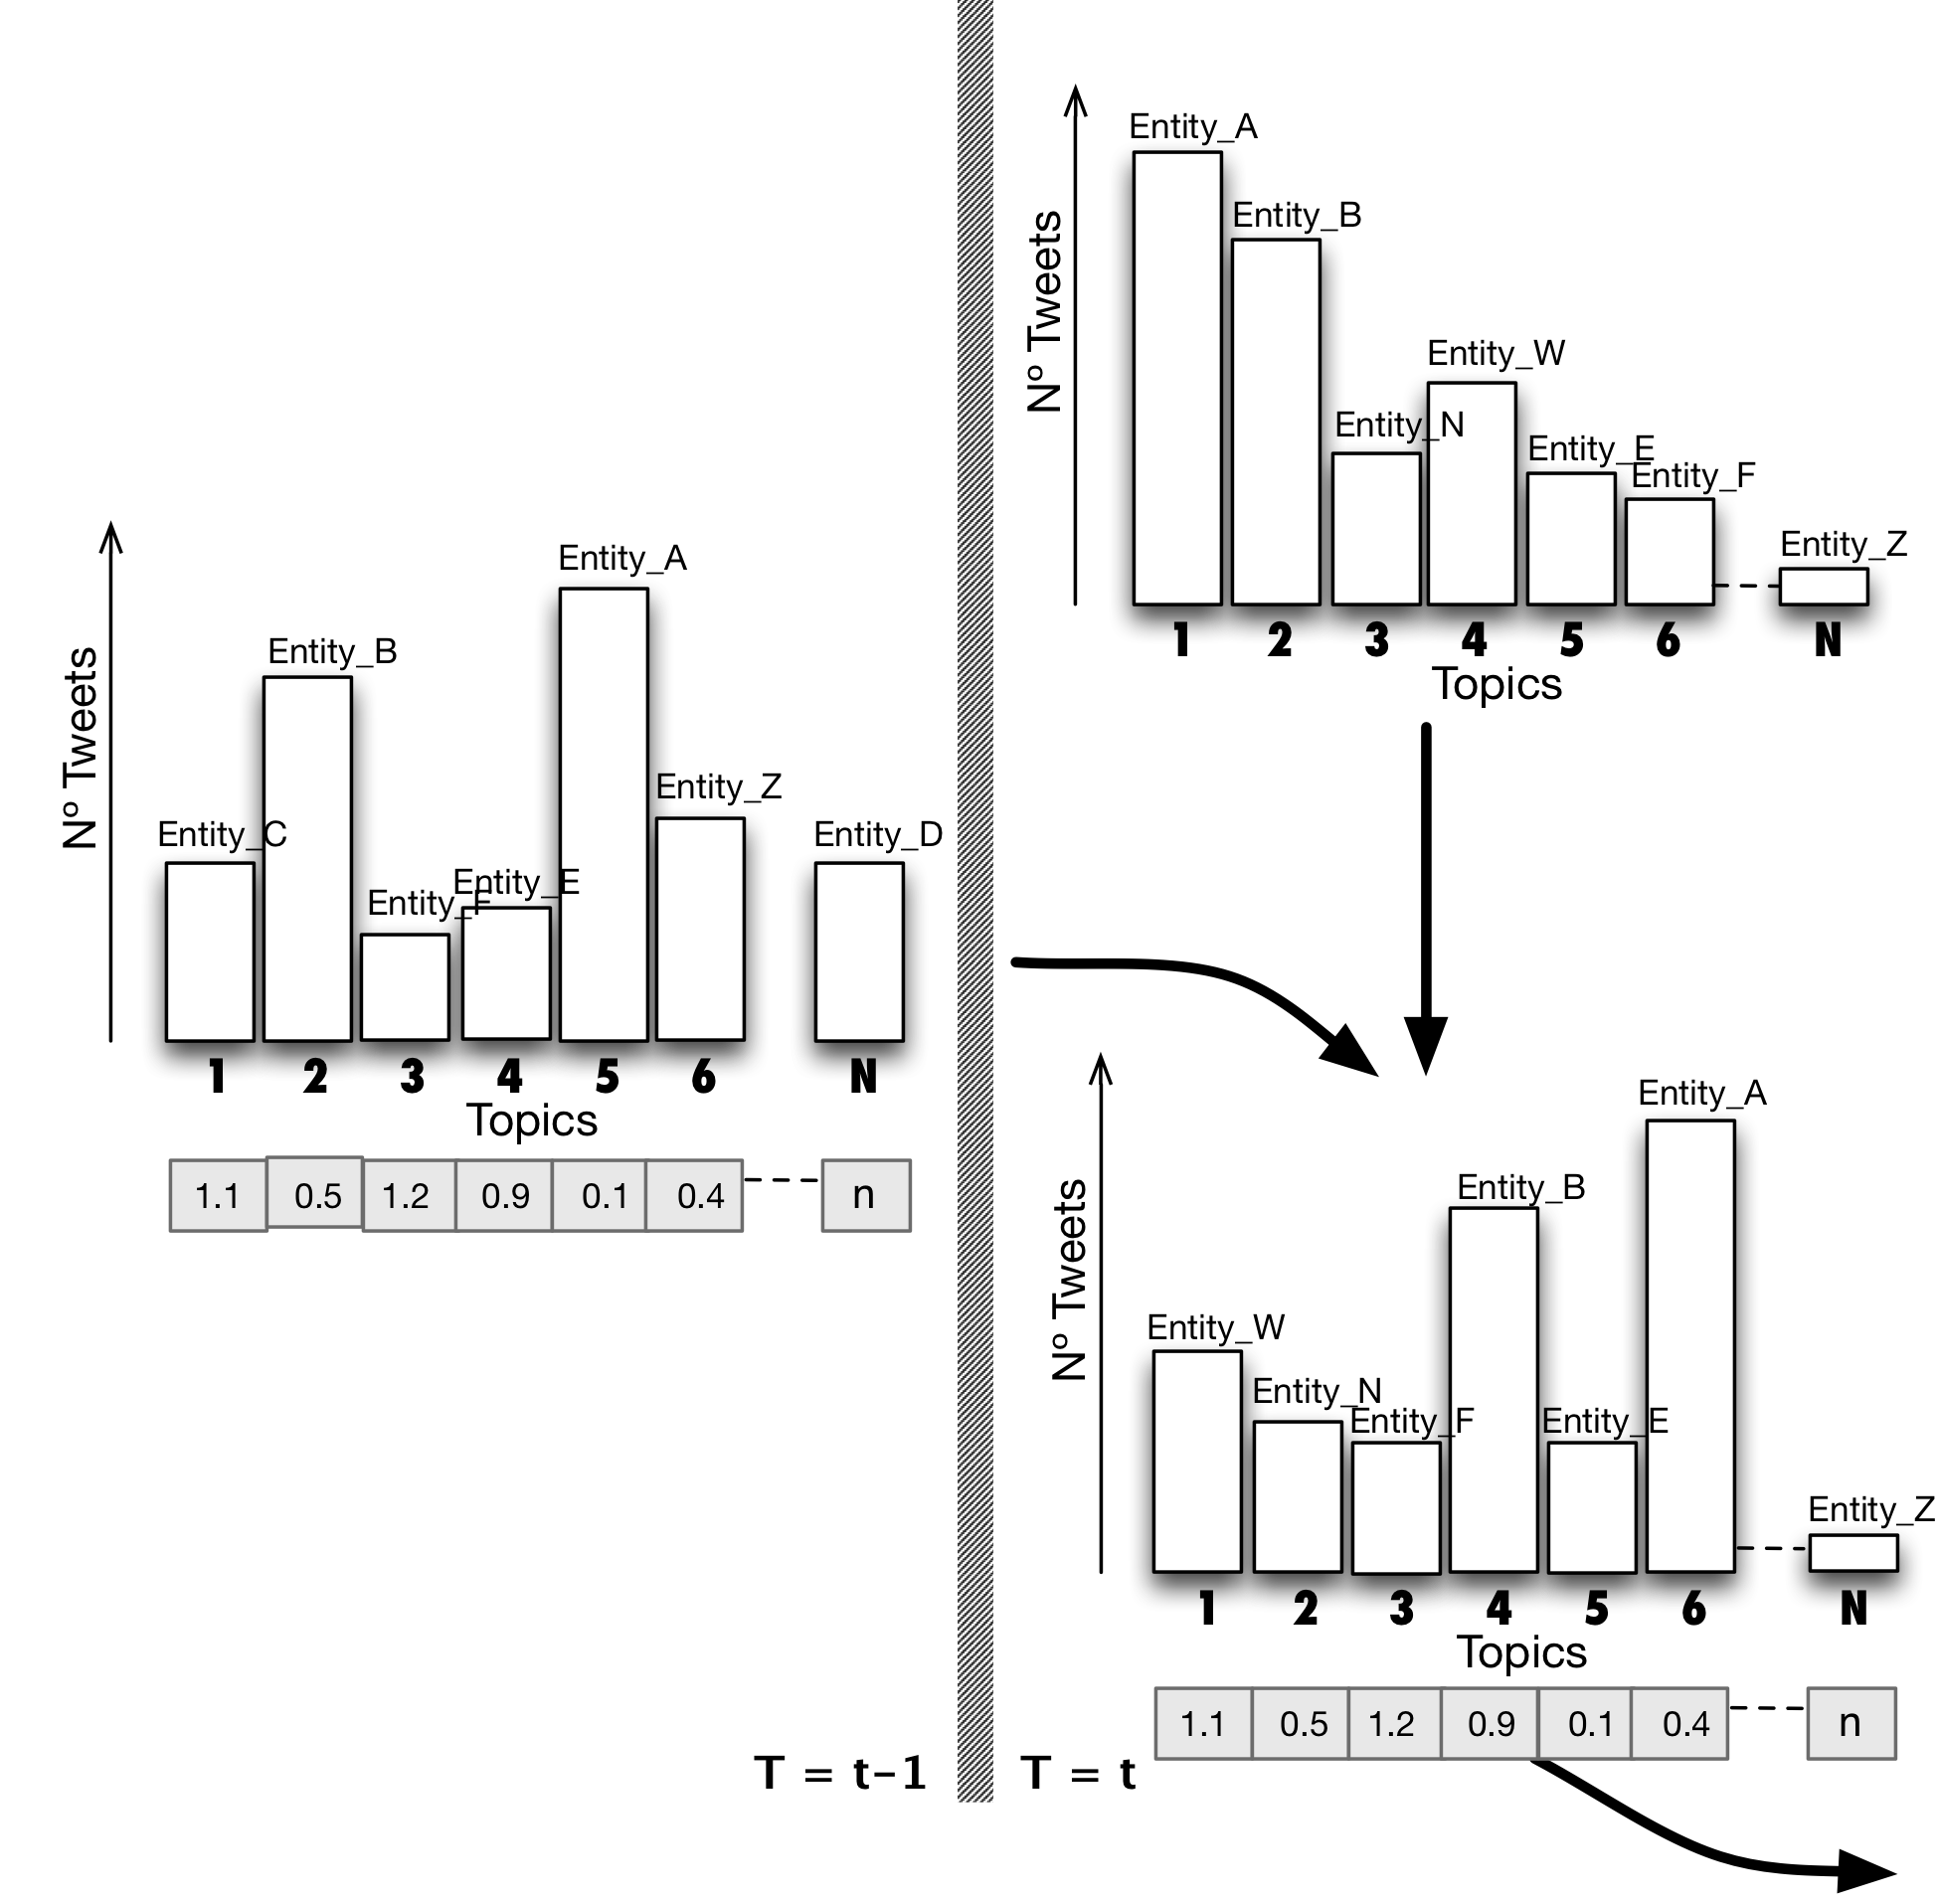
\includegraphics[width=0.5\textwidth]{figure/Tracking.png}
\caption{Using the evolution of previously calculated topics for reranking the present ones.}
\label{fig:Tracking}
\end{figure}

Even the topic relevance order is directly influenced by the scores from the last time-slot analysis and implicitly from the previous ones via the $V_{tendency}$ vector, the tracking logic could be further improved by explicitly considering more than one previous state, since more precise judges regarding the negative or positive slope of the tweet frequency curve could be done. Another intrinsic issue of any tracking approach is the \textit{cold start} problem: when analyzing the first time-slot for a particular event, we have no indications about how first data collected looked like before. This problem can be alleviated by increasing the temporal window via an early start of the collection process.

The algorithms for ranking clusters and the ones for tracking their changes in time should be closely tied in order to maximize the quality of the final topics. The different behavior of events make some approaches more suitable than others for certain kinds of events, but the way the accuracy of a topic detection varies for a particular kind of event is a research question that will not be studied in this paper.

\subsection{Exploiting Popularity}

In this phase we study the popularity of the clustered tweets in order to get extra insights about what are main event highlights and consequently re-rank the original set of candidate topics. Many possible dimensions can be considered for estimating the popularity of a certain status: number of relevant entities mentioned, presence of quality links pointing to other resources like videos or photos, usage of relevant hashtags, number of retweets, number of favorites... In this approach we will focus mainly in the two last ones since they provide a good estimation about the number of interactions derived this tweet has generated. Afterward we will be in a position to calculate the popularity of a certain cluster given the \textit{average tweet popularity} and the \textit{number of Peaks} inside.

\subsubsection{Tweet popularity}

Before globally analyzing the obtained topics we need to define a metric for calculating the popularity of a single tweet by considering together both retweets and favorites dimensions. We opted for a very simple combining logic consisting on a weighted sum of both variables. In order to decide about the most appropriate weights to be used, we analyzed a random set of 50.000 tweets randomly obtained from the collected tweets. For every tweet, we calculated the average ratio between the number of retweets and favorites, obtaining a final score of $3.92 \approx 4$. According to those findings, we have established the following equation:

\begin{equation}
\begin{split}
\text{Popularity}(tw) = \left |Retweets(tw)  \right | + 4*\left |Favorites(tw)  \right | \\
tw \in Tweets(Topic_N)
\end{split}
\end{equation}

\subsubsection{Peak Detection}

The peaks inside a particular time-slot are those individuals with an outstanding popularity over the average value. Considering the popularity of the tweets for a particular topic $Topic_N$ a normal distribution over the sample, we considerate as peaks those tweets whose popularity exceeded 2.5 times the corresponding standard deviation\footnote{\fontsize{8pt}{1em}\selectfont \url{http://en.wikipedia.org/wiki/Standard_deviation}}, which correspond approximately with a $2\%$ of the original population. In Figure~\ref{fig:Peaks} we can observe how only certain tweets with a high popularity compare to the average are selected as peaks. The rest of not so outstanding individuals are ignored in the current implementation of the popularity measure.

\begin{equation}
\begin{split}
\text{Peaks}(Topic_N) = \\
 \quad tw \in Topic_N : \text{Popularity}(tw) \geq 2*\sigma (Topic_N)
\end{split}
\end{equation}

\begin{figure}[h!]
\centering
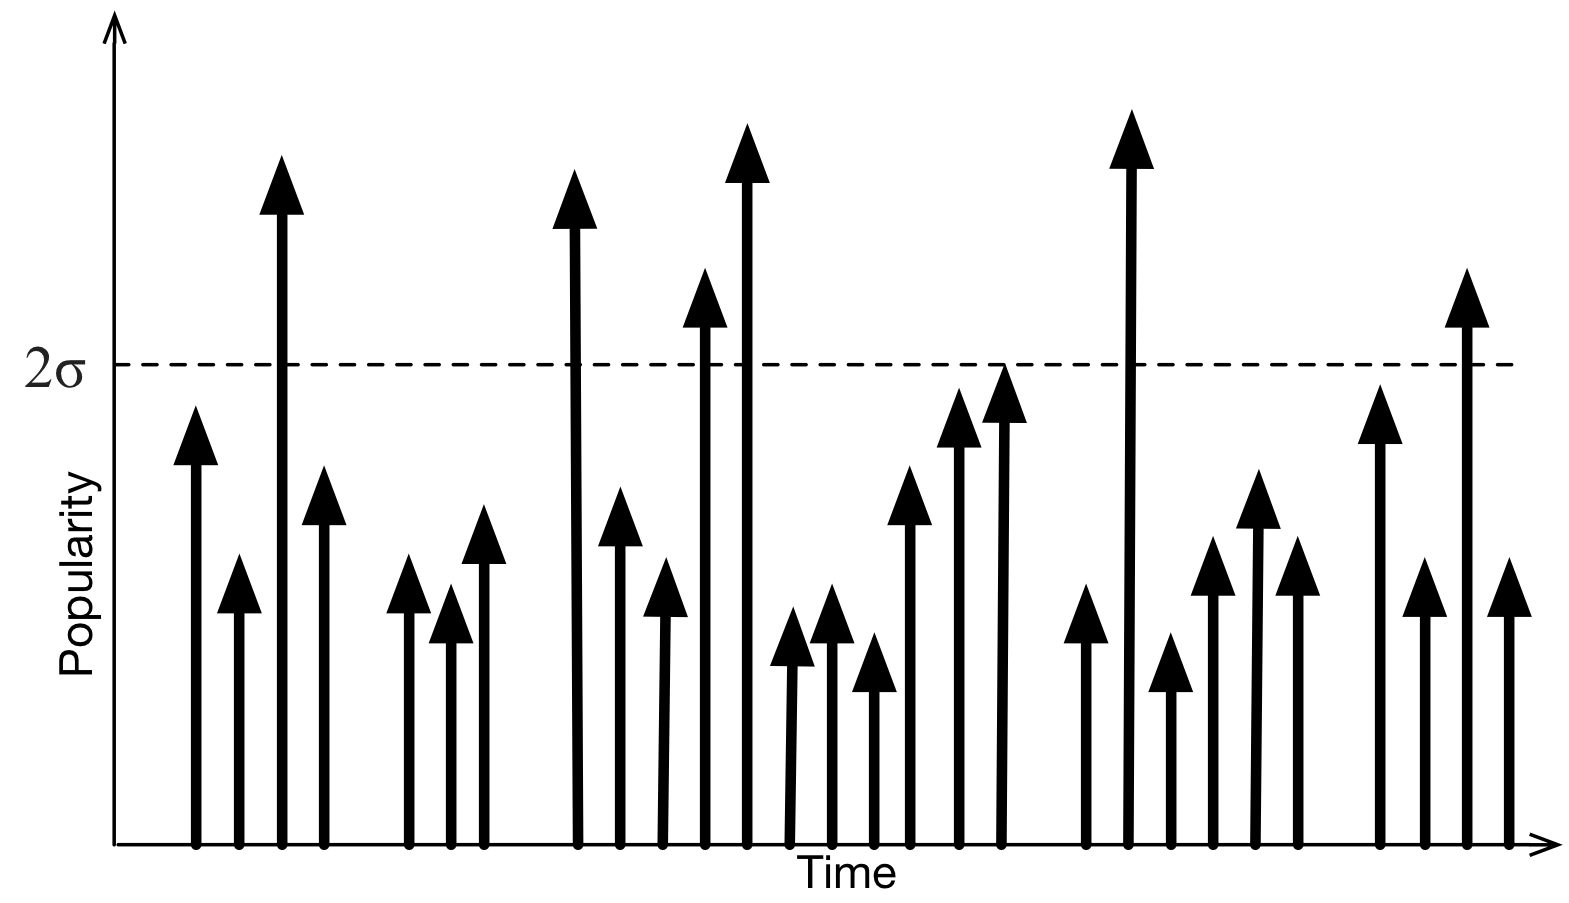
\includegraphics[width=0.4\textwidth]{figure/Peaks.png}
\caption{Detecting peaks inside a particular topic.}
\label{fig:Peaks}
\end{figure}

The same idea of studying the evolution of the topics in time should to be considered again in the case of the peaks. If we know about the tendency of a certain status in the past we can better consider it as a good candidate for the topic popularity measures or it should be relegated since it was something that had already repercussion in previous clusters. In our solution we opted for a very simple strategy consisting on annotating the peaks that have been already considered as outstanding in order to relax its popularity scores when they emerge again.

\begin{equation} \label{eq:topicpopularity}
\text{Pop}(Topic_N) =\left (\sum_{0}^{n}Popularity(tw)_i   \right )* \left |\text{Peaks}(Topic_N)  \right |
\end{equation}

In a last step, the number of peaks inside a certain topic and its average popularity are combined together as shown in Equation~\ref{eq:topicpopularity}, and the final score is used again for promoting certain topics over others inside a particular time-slot (popularity reranking) and for programmatically generating extra topic features like the ones shown in Section~\ref{sec:results}.

%%%%%%%%%%%%%%%%%%%%%%%%%%%%%%%%%%%
%%%  Results and Preliminary Evaluation  %%%
%%%%%%%%%%%%%%%%%%%%%%%%%%%%%%%%%%%

\section[Results and Preliminary Evaluation]{Results and Preliminary \\ Evaluation}
\label{sec:results}

Once the set of ranked clusters per each time-slot has been produced we are ready to produce the topics that become the final result of this approach. The first thing to be done is to filter the number of topics per time-slot. Since the output of the clustering operation produces many candidates that don't worth to be included in the output, a mechanism for discarding them is needed. In our case we ignore clusters whose relevance falls under a $90\%$ of the range of that particular time-slot. Then we use our knowledge about the corresponding topics for generating the following fields:
\begin{itemize}
  \item Beginning time/date of the time-slot where this topic belongs to.
  \item Topic title: human friendly sentence summarizing the main fact behind the topic. In our approach this field is obtained from the most relevant peak's text.
  \item Comma separated list of relevant tags. In our approach, we select other prominent entities inside the cluster.
  \item Id's of the main tweets inside the topic: list of tweet id's corresponding to peaks inside the cluster.
  \item List of Image: Valid image URL's mentioned in the tweets inside the cluster, ordered by the popularity of the tweets they belong to.
\end{itemize}

We have applied this method over two real scenarios.The first one corresponded to the United States presidential election of 2012 held on Tuesday, November 6, 2012, where the democratic nominee Barack Obama, and his running mate Vice President Joe Biden were re-elected to a second term, defeating the Republican nominee Mitt Romney. The organization of the Data Challenge~\cite{snow2014dc} provided a ground truth of topics to compare with, which were used for training purposes. For example Table~\ref{table:topics} shows some of the topics generated for the time-slot corresponding to the 07th at 00:40.

\begin{table}[tbp]
  \resizebox{8cm}{!} {
\begin{tabular}{ c | c | c | c | c | c }
  \hline
 Cluster\_Label & Tweets & EF & ECF & Peaks & $Rel_{Final}$  \\ \hline
dbpedia:United\_States\_presidential\_election &   193 &  185  &  0 & 8 & 0.9585492 \\
dbpedia:Democratic\_Party\_\%28United\_States\%29 &   165 &  146  &  1 & 9 &  0.8848484 \\
dbpedia:Republican\_Party\_\%28United\_States\%29 &   541 &  454 & 5 & 13 &  0.8391866 \\
dbpedia:Barack\_Obama & 1460 &  1165  &  17 & 21 &  0.7979452 \\
dbpedia:Kentucky &   163 &  126  &  1 & 25 &  0.77300613 \\
dbpedia:Virginia &   170 &  130  &  2 &  24 & 0.7647058 \\
dbpedia:Mitt\_Romney &   2458 &  1822  &  17 & 31 &  0.7412530 \\
dbpedia:United\_States &   185 & 131  &  0 & 12 & 0.7081081 \\
dbpedia:Ohio &   341 &  235  &  3 & 27 &0.6891495  \\
dbpedia:The\_Changing\_of\_Times & 921 &  603  &  6 & 3 &  0.6547231\\
dbpedia:Massachusetts &   363 & 237 & 1 &  16 &0.6528925\\
dbpedia:CNN & 211 & 136  &  1 &  9 & 0.6445497\\
dbpedia:George\_W.\_Bush &   172 &  109  &  0 & 13 & 0.6337209 \\
  \hline
\end {tabular}
  }
\caption{Proposed topics for a 10 minutes time interval corresponding to the American Elections 2012}
\label{table:topics}
\end{table}

The second experiment analyzed the difficult social and political situation in Ukraine and was conducted from the 17th Feb 2014 at 18:00 GMT to the 18th Feb at 18:00 GMT. The official evaluation results of our method in this particular data set are included in~\cite{snow2014dc}. However, we introduce here some general thoughts and first impressions. Regarding the textual labels of the generated topics, they seems to correspond to relevant facts occurring during those 24 hours. To judge if the time-slots where those topics have been included are indeed the correct ones is far more complicated since it is fuzzy to determine when a particular fact about an event should ideally show up. The comparison of the results with the clusters generated by applying LDA~\cite{Aiello} do not spread too much light about this neither. 

Other issue is the appearance of terms like market or Goldman Sachs that break the uniformity of the story. There is a reason for such irruption of economic domain concepts: the word "bitcoin" has been used as input during the streaming collection process. Whether this was made in purpose or not, it worths to be studied if the inclusion of terms concerning different matters still allows to correctly track the parallel stories happening, or if the noise introduced blurs the quality of the topic detection. 

The bigger size of the time-slots in the second experiment requires some changes through a more strict clustering filtering that avoids too large amount of candidate topics. Another difference of the current event against the training set was the volume of information generated: the American Elections is a really big event, condensed mainly in 24 hours, while the Ukrainian conflict do not have the same instant repercussion and lasts for several weeks instead. However, no changes seem to be needed in this line and both scenarios seem to be well analyzed under the same parameters. 

Going deeper into the topic features, entities seem to work pretty good as keywords, and the peak detection offers tweet Id's closely related to the topic matter. Labels are well readable, but we could have obtained more representativeness by applying some summarization techniques over the top N peaks instead of going for just the most popular tweet.


%%%%%%%%%%%%%%%%%%%%%
%%%  Conclusions  %%%
%%%%%%%%%%%%%%%%%%%%%

\section{Conclusions}
We presented an approach for automatically generating time-aware relevant topics about a particular event by harvesting posts coming from the Twitter Streaming API. After slicing the considered time interval in smaller time-slots, we rely on named entities recognized in tweets to spot hidden topics. Since frequent does not necessary mean relevant, we have weighted those results via inverse frequency measures and topic tracking over time. The resultant ranked list is finally completed with cues about the popularity of the tweets included in them. In particular, we promote clusters with high average topic popularity and larger number of peaks for outstanding tweets. Finally, we filter the ones with higher relevance and generate features that summarize the main highlights of this news event during the specified time period.

There are many open challenges for improving the current approach that we would like to further study in upcoming publications. First, something as simple as a preliminary text cleansing and reprocessing of the collected tweets may boost the final results, specially for those cases where we collect different tweets with almost the same text (some people just c\&p other tweets without retweeting or mentioning). Also, the current approach does not exploit all the rich metadata that Twitter is providing via the Streaming API. Instead of this, we operated over a reduced schema that ignores important fields like the so-called ''entities'' which contain mainly keywords and hashtags. Finally the entity cluster algorithm is based on a strict string similarity distance over the URLs. It could be interesting to study what happens when we adopt a more relax strategy involving some relative string measures such as the Jaro-Winkler string distance~\cite{winkler2006overview} over the labels. 

%ACKNOWLEDGMENTS are optional
\section*{Acknowledgments}
This research has been partially funded by the European Union's 7th Framework Programme via the project LinkedTV (GA 287911) and Ghent University.
%iMinds (Interdisciplinary institute for Technology) a research institute founded by the Flemish Government,
%the Institute for the Promotion of Innovation by Science and Technology in Flanders (IWT), the Fund for Scientific Research-Flanders (FWO-Flanders),

\bibliographystyle{abbrv}
\bibliography{snow_challenge}

\end{document} 